\section{Evaluation}
\label{sec:evaluation}

This section discusses the behaviour of our algorithm in the real
world.

Both for testing and for performance evaluation, we require a test
suite. We started with a carefully crafted, manually produced, suite
of valid and invalid tests. This test suite was constructed by
gathering pairs of types that emerged from examples we have studied
and from programs we have written in FreeST, the programming language
for context-free session
types~\cite{almeida.etal_freest-functional-language}.
% This suite comprised of a total os 169 valid and invalid tests.  The
% primary purpose of this preliminary evaluation step was to confirm
% the algorithm would be able to handle manual examples that we knew
% would emerge from real programs and examples. The algorithm
% succeeded in evaluating all the tests in due time.
The tests produced by this method are, on the one hand, small, and, on
the other hand, lacking diversity.

We then turned our attention to the automatic generation of test
cases. Generating pairs of arbitrary (well-formed) types that share no
variables is simple. The difficulty lies in deciding whether two such
types, independently generated, are bisimilar. Even if an oracle could
be identified, the probability that a randomly generated pair of types
turns out to be equivalent would be extremely low. Instead, we proceed
by generating arbitrary pairs of types that are bisimilar by
construction. Theorem~\ref{thm:axioms} naturally induces an algorithm:
given a natural number $n$ (the size of the pair), arbitrarily select
for the base case ($n=0$) one of the pairs in item 1 of the theorem
and for the recursive case ($n\ge1$) one of the pairs in 2--12 items.

\begin{theorem}[Properties of type equivalence]
\label{thm:axioms}
  \begin{enumerate}
    % Congruence
  \item $\skipk \TypeEquiv \skipk$ and $\sharp B \TypeEquiv \sharp B$;
  \item $S;T \TypeEquiv U;V$ if $S \TypeEquiv U$ and $T \TypeEquiv V$;
  \item $\mu X.S \TypeEquiv \mu X.T$ if $S \TypeEquiv T$;
  \item $\star\{\ell_i\colon S_i\}_{i\in I}\TypeEquiv
    \star\{\ell_i\colon T_i\}_{i\in I}$ if $(S \TypeEquiv T)_{i\in
      I}$;
    % Laws for sequential composition
  \item $S\TypeEquiv T;\skipk$ and $S\TypeEquiv \skipk;T$ if $S \TypeEquiv T$;
  \item $\star\{\ell_i\colon S_i\}_{i\in I};U\TypeEquiv
    \star\{\ell_i\colon T_i;V\}_{i\in I}$ if $(S_i \TypeEquiv T_i)_{i\in
      I}$ and $U \TypeEquiv V$;
  \item $T \TypeEquiv S$ if $S \TypeEquiv T$;
  \item $R;(S;T) \TypeEquiv (U;V);W$ if $R \TypeEquiv U$, $S \TypeEquiv V$, and $T\TypeEquiv W$;
    % Laws for mu-types
  \item
    $\mu X.\mu Y.S \TypeEquiv \mu X.\subs XYT \TypeEquiv \mu Y.\subs
    YXT$ if $S \TypeEquiv T$;
  \item $\mu X.S \TypeEquiv T$ if $S \TypeEquiv T$ and $x\notin\free(S)$;
  \item $\subs UXS\TypeEquiv \subs VXT$  if $S \TypeEquiv T$ and $U \TypeEquiv V$;
  \item $\mu X.S \TypeEquiv \subs{\mu X.T}{X}T$ if $S \TypeEquiv T$.
  \end{enumerate}
\end{theorem}
%
\begin{proof}
  1--3: Bisimulation is a congruence. 4--12: Thiemann and
  Vasconcelos~\cite{thiemann2016context} exhibit the appropriate
  bisimulations.
\end{proof}

For evaluating the algorithm on non-bisimilar pairs we independently
generate two types, run function $\BisimT$ on them, and discard the
data collected in the rare event that the pair turns out to be
bisimilar.
%
For testing, however, we rely on manually crafted tests, given that a
solution based on anti-axioms does not work: bisimulation for
context-free session types is such that there are types
$S \not\bisim T$ such that $\mu X.S \bisim \mu X.T$ (just think of
$!\intk;X;X$ and $!\intk;X$).

We used QuickCheck~\cite{DBLP:conf/icfp/ClaessenH00} generate two test
suites. That for bisimilar pairs (constructed based on
Theorem~\ref{thm:axioms}) comprises 1000 entries, featuring types with
a number of nodes (in the syntax tree) ranging from 1 to 35751. The
test suite for non-bisimilar pairs (constructed by independently
generating two types and verifying they were not equivalent) includes
1000 pairs with a number of nodes ranging from 1 to 387.
%
The slowest negative test takes under 775Mb of RAM to execute.

The base algorithm described in the previous section turns out to
behave quite poorly. We then implemented the
following variants:
%
\begin{enumerate}
\item \emph{Eliminating redundant productions in the grammar.}
  Realising that the size of the expansion tree depends, among other
  things, on the number of productions in the grammar, we looked into
  ways of generating smaller grammars. Rather than blindly adding a
  new production $Y \rightarrow \vec Z$, we look, in the set of
  productions, for a production $W \rightarrow \vec X$ such that the
  language generated from $\vec Z$ coincides with that from $\vec
  X$. In this case, we add no new production and return
  non-terminal~$W$ instead. To find~$W$, we look for the least
  fixed-point of the transitions in the languages generated by
  $\vec Z$ and $\vec X$ and compare them.
  \item
  \emph{Using a filter rule that removes nodes with hopeless pairs.} A
  filter rule ensures that nodes composed by pairs of types with
  different norms (if normed) are removed from the expansion tree,
  since these types are not equivalent.  Notice that the filter rule
  preserves the results of soundness and completeness.
  \item
  \emph{Using a double-ended queue to prepend promising children.} A
  double-ended queue allows prioritizing nodes with potential to reach
  an empty node faster.  The algorithm prepends (rather than appends)
  empty nodes or nodes whose pairs $(\vec X, \vec Y)$ are such that
  $|\vec X|\leq 1$ and $|\vec Y| \leq 1$.
  \item
  \emph{Iterating the simplification stage until a fixed point is
    reached.} Iterating the simplification procedure on a given node
  $N$, the algorithm computes the simplest possible children nodes
  derived from $N$. We showed that the simplification function that
  results from applying the reflexive, congruence, \BPA, and filter
  rules, has a fixed point in the complete partial ordered set of
  pairs node-ancestors, where the set of ancestors is fixed.
\end{enumerate}

To better understand how the algorithm performs in practice, we tested
all the variants. We evaluated each variant 1--4 individually (denoted
by B1--B4) and the gradual inclusion of variants, by the
order in which they were introduced above (cases B12, B123, B1234).
B0 stands for the base algorithm, $\BisimT$.
%
  We implemented the base algorithm and its
  variants %described by the function $\BisimT$
  in Haskell, using the Glasgow Haskell Compiler (version 8.6.5). % We also
  % implemented the optimisations 1-4 above.
  The evaluation was conducted on a machine with an Intel Core i7-6700K at
  4.2GHz and 8 GB of RAM running Arch Linux; tests were run under a timeout
  of 2 minutes.

For B0 we had 5 tests exceeding the timeout, for B1--B4 the number of timeouts
ranged from 1 to 12, for B12 we had 2 timeouts, whereas for B1234 all tests
ran in less than 30 minutes. 
%
%\begin{table}
%\centering
%	\begin{tabular}{ |c|c|c|c| }
%	 \hline
% 		Version ID & Version description & Bisimilar test suite & Not bisimilar 
% 		test suite \\ 
% 		 \hline
%	 	B0 & \text { base case}& 5 & 0 \\  
%	 	B1 & \text { reuse productions}& 2 & 1 \\ 
%	 	B2 & \text { use double-ended queue}& 6 & 0 \\ 
%	 	B3 & \text { use filtering}& 12 & 0 \\
%	 	B4 & \text { iterate simplification}& 4 & 0 \\
%	 	B12 & \text {case B1 + case B2}& 3 & 1 \\   
%	 	B123 & \text {case B12 + case B3}& 7 & 1 \\
%	 	B1234 & \text {case B123 + case B4}& \bf{1} & \bf{1} \\ 
%	 	 \hline  
%	\end{tabular}
%	\caption{Number of timeouts for each optimisation.\label{table:timeouts}}
%\end{table}
%
%
Figure~\ref{fig:results} (a) depicts the distribution of the execution
times (in $\mu s$) for both test suites and for all optimisations.  In
this plot, we observe the distribution of tests for each execution
time.  All the versions exhibit similar execution times for the
majority of the tests.   
%
Figure~\ref{fig:results} (b) represents the distribution of execution
time per total number of nodes in the abstract syntax trees of the
types. We observe an exponential increase in the runtime.
%
Although we have carried out tests with a
fairly large number of nodes in their abstract syntax trees, we remark
that, when used in a compiler, the algorithm will mostly come across
types with a reduced number of nodes.


\begin{figure}[t]
    \centering
    \subfloat[Distribution of the execution time]{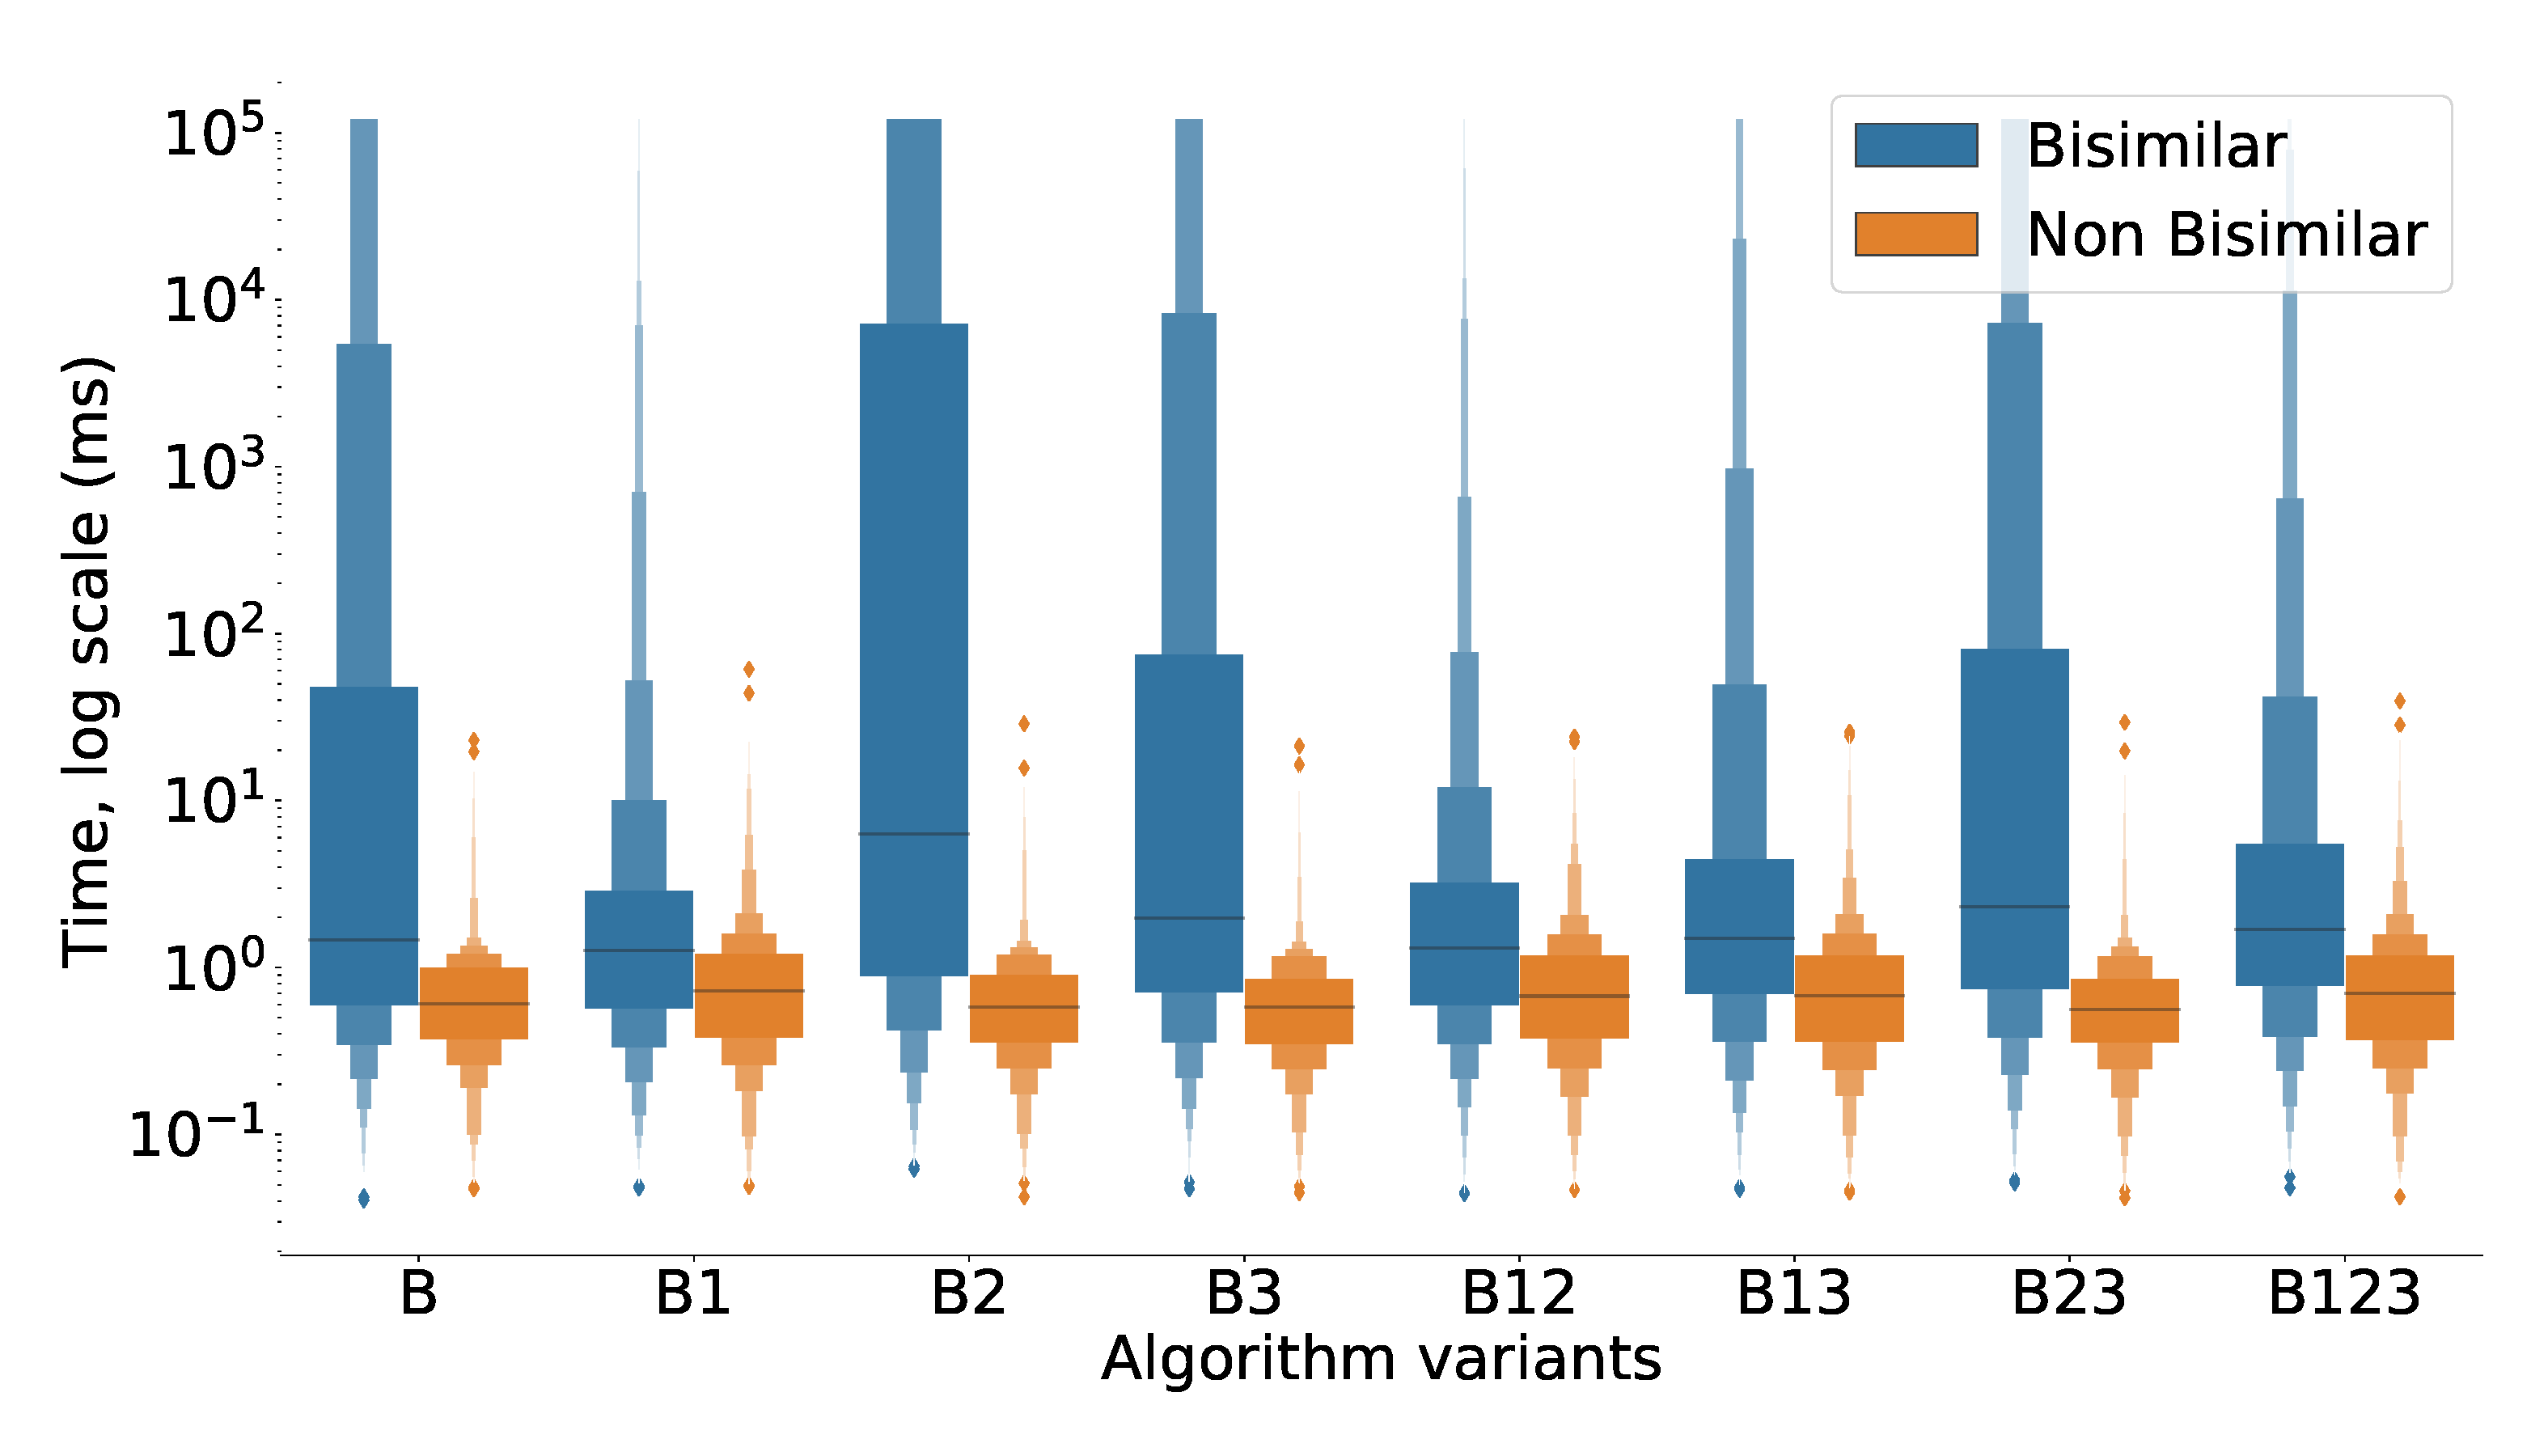
\includegraphics[height=.5\textwidth]{img/distribution_boxplot}}%
    \subfloat[Execution time per number of nodes]{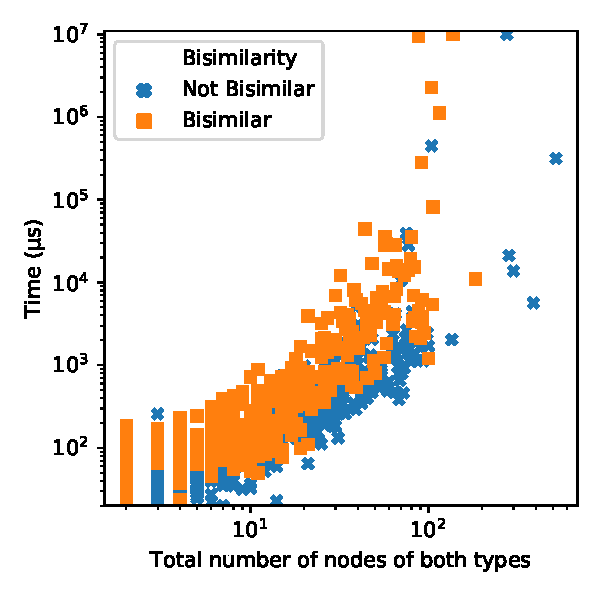
\includegraphics[height=.5\textwidth]{img/nodes_time_B1234}}%
    \caption{The test suite composed by equivalent pairs of types is represented in orange and the
    test suite with non-equivalent pairs of types is represented in blue. Time 
    in microseconds, $\mu s$. Both scales are logarithmic.\\
    (a) Distribution of execution time of function $\BisimT$ for both test suites.\\
    (b) Distribution of execution time of function $\BisimT$ per total number of nodes 
    in the abstract syntax trees of the types.}%
    \label{fig:results}%
\end{figure}


%\noindent
%\begin{minipage}[b]{0.49\textwidth}
%   {\small 
%  \centering
% 	\begin{tabular}{ |c|c|c| }
%	 \hline
% 		Version &  {\color{orange}Bisimilar} & {\color{MidnightBlue}Not bisimilar}  \\ 
% 		 \hline
%	 	B0 & 5 & 0 \\  
%	 	B1 &  1 & 0 \\ 
%	 	B2 & 6 & 0 \\ 
%	 	B3 &  12 & 0 \\
%	 	B4 &  4 & 0 \\
%	 	B12 &  2 & 0 \\   
%	 	B123 &  6 & 0 \\
%	 	B1234 &  \textbf{0} & \textbf{0} \\ 
%	 	 \hline  
%	\end{tabular}\vspace*{6mm}
%	\captionof{table}{Number of timeouts for each optimisation and for both test 
%	suites.\label{table:timeouts}\vspace*{4mm}}
%	}
%	\end{minipage}
%	\hfill
%\begin{minipage}[b]{0.49\textwidth}
% {\small 
%\centering
%    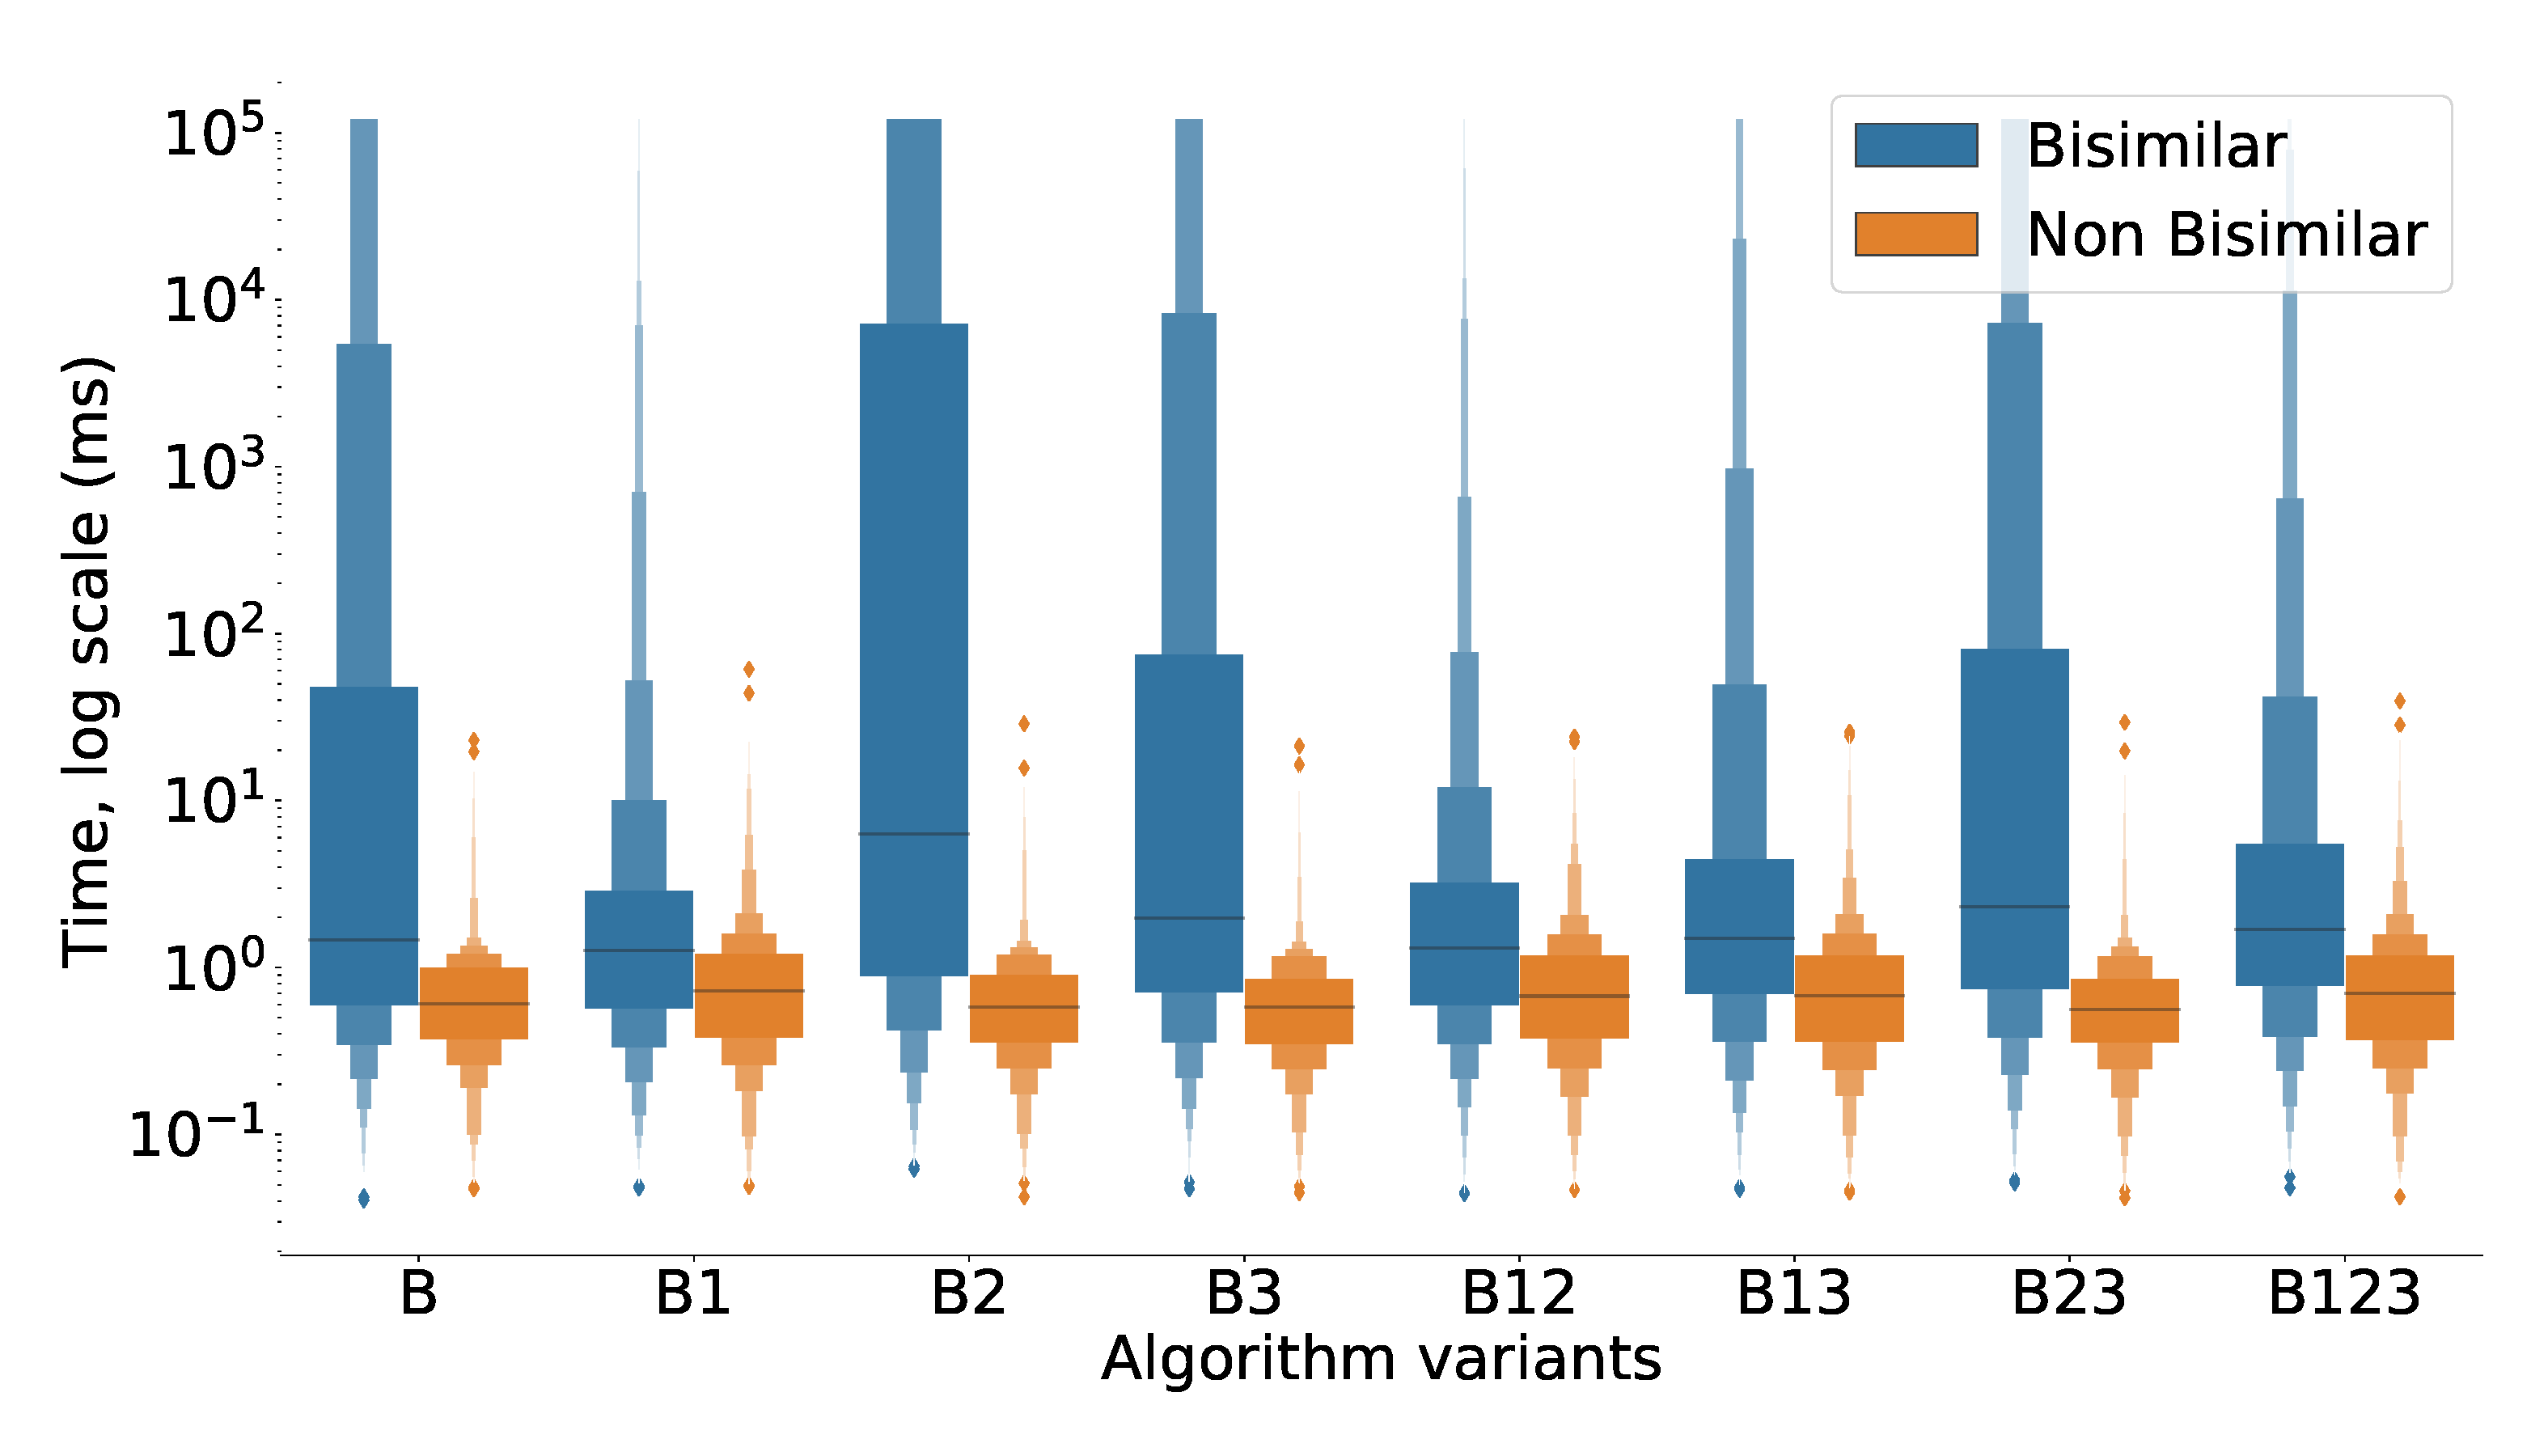
\includegraphics[height=.85\textwidth]{img/distribution_boxplot}%
%    \captionof{figure}{Distribution of execution time of function $\BisimT$ for both test suites. 
%    Both scales are logarithmic.\label{fig:results}}}
%    %\caption{Distribution of the execution time. \label{fig:results}}
%\end{minipage}

%%% Local Variables:
%%% mode: latex
%%% TeX-master: "main"
%%% End:
